\begin{conclusion} \label{conclusion}

Závěrem lze říci, že vytvořená aplikace má před sebou ještě dlouhou cestu svého vývoje, avšak její základ je vytvořen na stabilním podkladu, ze kterého bude možné ji dále efektivně rozvíjet. Návrhy na další funkce, které buďto nebyly zcela dokončeny v rámci této práce, nebo které byly objeveny až při jejím uživatelském testování, jsou evidovány v systému Trello.\\
Během realizace jsem se naučil alespoň na určité úrovni používat framework Vue.js, který se mi během tohoto procesu velmi zalíbil, a jistě jej použiji i v jiných projektech. Kromě této technologie jsem také více pronikl do architektury moderních frontendových aplikací, u kterých může být výzvou řešení konektivity, rychlosti načítání obsahu nebo jejich kompatibilita se zastaralými prohlížeči.\\
Výsledná aplikace, tak jak je k dispozici při dokončování tohoto textu, je reálně použitelná - obsahuje nezbytná zabezpečení jako například OAuth2 přihlašování nebo podporu čtečky kódů. Přesto ještě před jejím reálným nasazením doporučuji vylepšit některé klíčové funkce, u kterých z uživatelského testování vzešly podněty ke zlepšení.
V průběhu celé práce jsem si zaznamenával čas strávený realizací tohoto projektu, který nyní jako měsíční souhrny přikládám v grafu \ref{picture:time:spent}.

\begin{figure}[H]
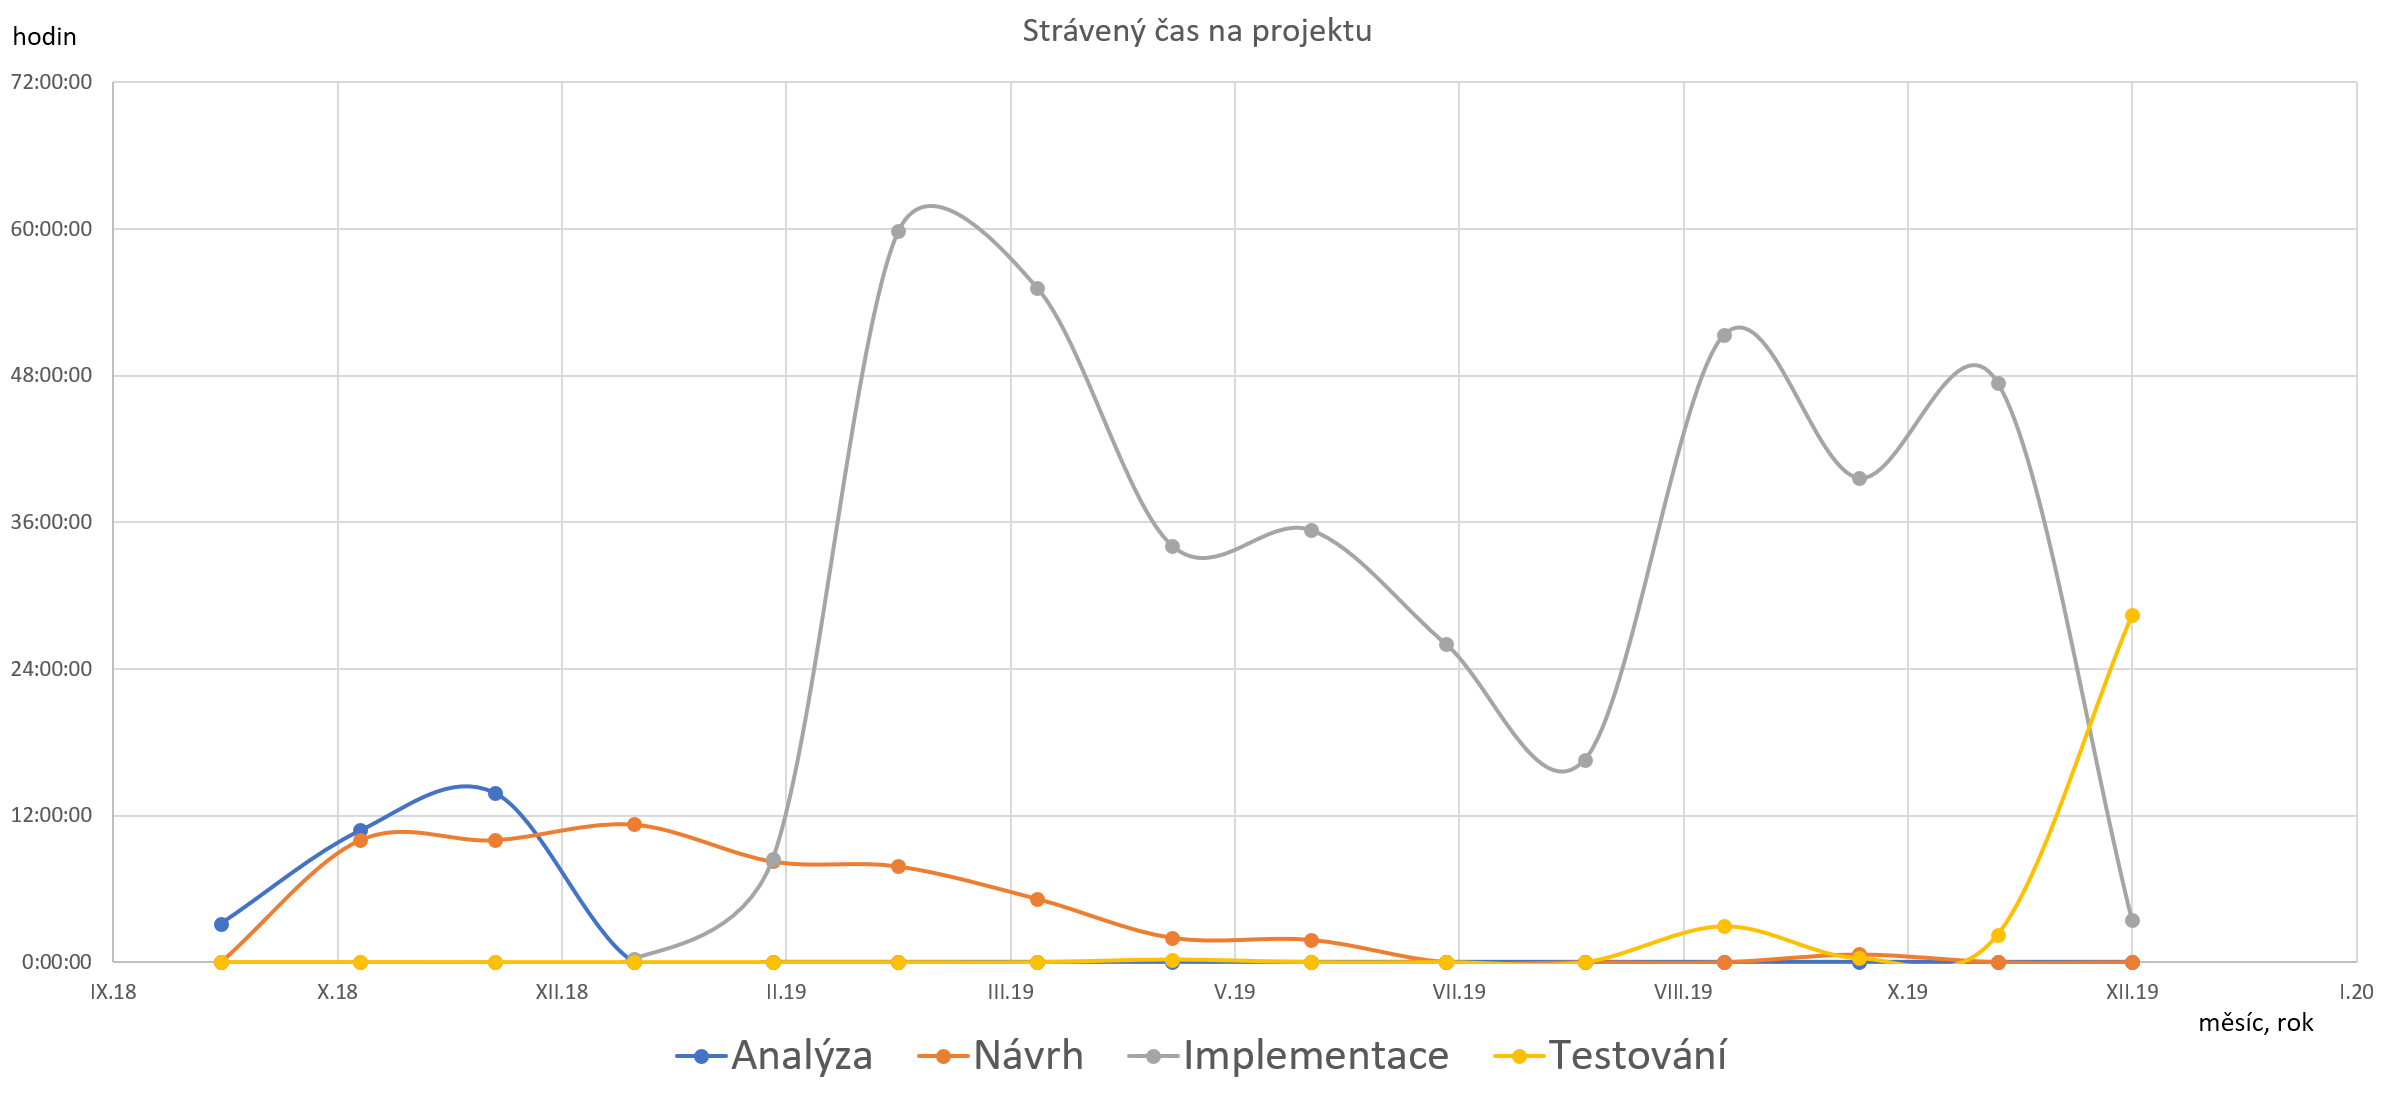
\includegraphics[width=0.9\textwidth]{../png/time/time_spent.png}
\caption[Měsíční čas strávený realizací projektu]{Čas strávený realizací projektu, rozdělený dle typu aktivity.} \label{picture:time:spent}
\end{figure}

Při zpětném ohlédnutí na tento graf vidím poměrně velkou převahu implementační části, která je způsobena tím, že analýzu jsme prováděli ještě ve dvou - společně s Pavlem Kovářem, a její efektivita byla poměrně vysoká. Naopak zejména počátky implementace, které spočívaly převážně v učení se pro mě zcela nové technologie, přinesly pochopitelnou neefektivitu samotného vývoje a tudíž nárůst stráveného času.\\
Testování eviduje rapidní nárůst až v závěru, což je způsobenou velkou časovou náročností uživatelského testování ve skladech. Přesto bylo testování realizováno i průběhu vývoje, avšak oproti závěru to bylo ve velmi malé míře.\\

\end{conclusion}
